%%%%%%%%%%%%%%%%%%%%%%%%%%%%%%%%%%%%%%%%%
% Beamer Presentation
% LaTeX Template
% Version 1.0 (10/11/12)
%
% This template has been downloaded from:
% http://www.LaTeXTemplates.com
%
% License:
% CC BY-NC-SA 3.0 (http://creativecommons.org/licenses/by-nc-sa/3.0/)
%
%%%%%%%%%%%%%%%%%%%%%%%%%%%%%%%%%%%%%%%%%

%----------------------------------------------------------------------------------------
%	PACKAGES AND THEMES
%----------------------------------------------------------------------------------------

\documentclass[10pt,handout]{beamer}
% \documentclass[10pt]{beamer}

\usepackage{fouriernc}
\usepackage{amsmath}
\usepackage{amssymb}
\usepackage{mathtools}
\usepackage{xcolor}
\usepackage[utf8]{inputenc}
\usepackage[T1]{fontenc}
\usepackage{textcase}


\mode<presentation> {

% The Beamer class comes with a number of default slide themes
% which change the colors and layouts of slides. Below this is a list
% of all the themes, uncomment each in turn to see what they look like.

%\usetheme{progressbar}
%\progressbaroptions{headline=sections}

\usetheme{Darmstadt}
% \usecolortheme{albatross}
% \usecolortheme{beaver}
% \usecolortheme{beetle}
% \usecolortheme{crane}
% \usecolortheme{dolphin}
% \usecolortheme{dove}
% \usecolortheme{fly}
% \usecolortheme{lily}
% \usecolortheme{orchid}
% \usecolortheme{rose}
% \usecolortheme{seagull}
% \usecolortheme{seahorse}
% \usecolortheme{whale}
% \usecolortheme{wolverine}

%\setbeamertemplate{footline} % To remove the footer line in all slides uncomment this line
%\setbeamertemplate{footline}[page number] % To replace the footer line in all slides with a simple slide count uncomment this line

%\setbeamertemplate{navigation symbols}{} % To remove the navigation symbols from the bottom of all slides uncomment this line
}

\usepackage{graphicx} % Allows including images
\usepackage{booktabs} % Allows the use of \toprule, \midrule and \bottomrule in tables

\setbeamercovered{dynamic}
\definecolor{dgreen}{rgb}{0.,0.6,0.}
\newcommand{\beispiel}[1]{\textcolor{dgreen}{\textbf {#1}}}


%----------------------------------------------------------------------------------------
%	TITLE PAGE
%----------------------------------------------------------------------------------------

\title[RoBO]
{Robust Bayesian Optimization}
 % The short title appears at the bottom of every slide, the full title is only on the title page


\author{Joel Kaiser, José Luis Licón}
\institute[Uni Freiburg] % Your institution as it will appear on the bottom of every slide, may be shorthand to save space
{
Albert-Ludwigs-Universität Freiburg \\ % Your institution for the title page
\medskip
% \textit{liconj@informatik.uni-freiburg.de} % Your email address
}
\date{\today} % Date, can be changed to a custom date

\begin{document}
\setbeamertemplate{caption}{\insertcaption}



\begin{frame}
\titlepage % Print the title page as the first slide
\end{frame}

\begin{frame}
\frametitle{Overview} % Table of contents slide, comment this block out to remove it
\tableofcontents % Throughout your presentation, if you choose to use \section{} and \subsection{} commands, these will automatically be printed on this slide as an overview of your presentation
\end{frame}

%----------------------------------------------------------------------------------------
%	PRESENTATION SLIDES
%----------------------------------------------------------------------------------------

%------------------------------------------------
\section{Introduction}



%------------------------------------------------

%------------------------------------------------
% \section{Theoretical background}

%------------------------------------------------
%
%\subsection{Bayesian Optimization}
%
%
%\begin{frame}
%\frametitle{Problem description}
%
%In an optimization problem one looks for extrema of the form
%
%\[
%	\max \left\{ f(x) \mid x \in \mathcal A \subset \mathbb{R}^n \right\},
%\]
%subject to various conditions on $f : \mathbb{R}^n \rightarrow \mathbb{R}$ and
%$\mathcal{A} $.
%
%Assume the analytic form of $f$ is unknown, and our current knowledge
%about it can be described by a probability measure $P(f)$ defined over a 
%suitable function space. 
%
%Furthermore, let 
%\[
% \mathcal{D}_{1:t} = \left\{ x_1 , \ldots, x_t, f(x_1), \ldots , f(x_t) \right\}
%\]
%be a set of accumulated evaluations of $f$. 
%\end{frame}

%------------------------------------------------


%------------------------------------------------
%\begin{frame}
%\frametitle{Problem description}
%
%Then our posterior distribution over
%the space of functions will be described by
%\[
%	P(f \mid \mathcal{D}_{1:t}) \propto P( \mathcal{D}_{1:t} \mid f) P(f)
%\]
%
%The cenrtal problem in Bayesian optimization thus becomes using this posterior
%distribution to select a new point $x_{t+1} \in \mathcal{A}$ to sample. To do
%this efficiently, an acquisition function is employed.
%
%Once the new function value is observed, the set $\mathcal{D}_{1:t+1}$ is
%constructed and used to obtain a new posterior distribution. This process 
%can be continued until convergence is achieved.
%\end{frame}
%------------------------------------------------



%------------------------------------------------

\section{Entropy Search}

\begin{frame}
\frametitle{Problem definition}

Main idea: maximize information gain from succesive evaluations of an objective 
function.

% Let $I \subset \mathbb R^D$ be a bounded set, and $f : I \rightarrow \mathbb{R}$
% a (possibly unknown) function. A probability measure $p(f)$ over the function
% space $\mathbb{R}^I$ will in turn induce the following probability measure:
% 
% \[
%   p_{min}(x) \coloneqq P \left\{ x = \arg\!\min f(x) \right\} = 
%   \int_{f: I \rightarrow \mathbb{R}} p(f) \, 
%     \prod_{\widetilde x \in I} H[f(\widetilde{x} - f(x)] df
% \]
% 
% The objective will be to obtain a maximally informative probability measure
% after a number $n$ of function evaluations. This problem is rendered 
% computationally tractable by making several approximations. 
% \begin{columns}[c] % The "c" option specifies centered vertical alignment while the "t" option is used for top vertical alignment


% \column{.6\textwidth} % Right column and width

% \scalebox{10}{\textbf{*}}


\end{frame}
%------------------------------------------------


%------------------------------------------------
 
\begin{frame}
\frametitle{Problem definition}

\begin{itemize}
	\item $p(f)$ is defined as a Gaussian process
	\item $p_{min}$ is discretized to a set of representer points chosen from
	a non-uniform measure
	\item $p_{min}$ is approximated, either by expectation propagation
	or a Montecarlo method
	\item The change in $p(f)$ as a function of the next function evaluation
	can be predicted using the Gaussian process
	\item Relative entropy w.r.t. a uniform distribution is chosen as a loss
	function
	\item Expected information gain from future evaluations can be 
	approximated via the loss function
	\item The locations for new evaluations are evaluated greedily
\end{itemize}

\end{frame}
%------------------------------------------------

%------------------------------------------------
\begin{frame}
\frametitle{Discrete representation of continuous distributions}

This methods for this are contained in the \emph{sampling} module.

\begin{itemize}
  \item \emph{sample\_from\_measure}
  (model, xmin, xmax, n\_representers, BestGuesses, acquisition\_fn). Produces 
  a set of representer points based on the values of the chosen acquisition 
  function.
  
  \item \emph{slice\_ShrinkRank\_nolog}(xx, P, s0, transpose). An implementation
  of slice sampling.
\end{itemize}


\end{frame}
%------------------------------------------------

%------------------------------------------------
\begin{frame}
\frametitle{Expectation Propagation}

\begin{itemize}
  \item 1.
\end{itemize}


\end{frame}
%------------------------------------------------

%------------------------------------------------
\begin{frame}
\frametitle{Expected Information Gain}

This is evaluated in the \emph{dh\_fun} method within the \emph{Entropy} module:

\begin{itemize}
  \item \emph{dh\_fun}(self, x, invertsign=True, derivative=False)
  \item This can supply the numerical derivatives of the entropy function

\end{itemize}


\end{frame}
%------------------------------------------------



%------------------------------------------------
\begin{frame}
\frametitle{EntropyMC}

\begin{itemize}
  \item \emph{calc\_pmin}(self, f)
  \item \emph{change\_pmin\_by\_innovation}(self, x, f). The covariance matrices
  involved quickly become ill-conditioned.
  \item \emph{dh\_fun}(self, x): calculates the K-L divergence with respect to
  the approximation of $p_{min}$.
\end{itemize}

\end{frame}
%------------------------------------------------


%------------------------------------------------
\section{RoBO}

\subsection{Architecture}

%------------------------------------------------
\begin{frame}
\frametitle{Main modules}

\begin{center}
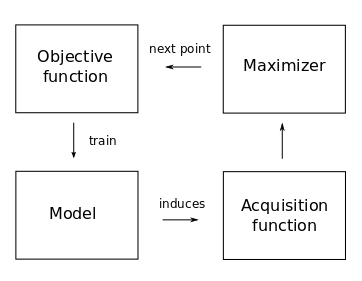
\includegraphics[width=0.7\textwidth]{robo_framework.png}
\end{center}


\end{frame}
%------------------------------------------------

%------------------------------------------------
\begin{frame}
\frametitle{Models}
\begin{itemize}
\item API
\begin{itemize}
\item \textit{train(X, Y)}. Trains model
\item \textit{update(X, Y)}. Updates the model
\item \textit{predict(X)}. returns mean and variance
\item \textit{predict\_variance(X1, X2)}. Returns part of covariance matrix for information gain
\item \textit{sample(X, size=10)}. Samples at X
\end{itemize}
\item Implementations:
\begin{itemize}
\item \textit{GPyModel} A wrapper to GPy.GPRegression
\end{itemize} 
\end{itemize}
\end{frame}
%------------------------------------------------

%------------------------------------------------
\begin{frame}
\frametitle{Acquisition functions}
\begin{itemize}
\item API
\begin{itemize}
\item \textit{\_\_init\_\_(model, X\_lower, X\_upper)}. As constructor
\item \textit{\_\_call\_\_(X, derivative=False)}. Returns some real number for all X
\item \textit{update(model)}. Should be called before getting maximized
\end{itemize}
\item Implementations:
\begin{itemize}
\item \textit{Expected Improvement}. Returns derivatives.
\item \textit{log(EI)}. Supports only one dimensional inputs, returns derivatives.
\item \textit{Probability of improvement}. Returns derivatives.
\item \textit{Upper confidence bound}. Not well tested.
\item \textit{Entropy Search}. EP-based information gain of the probability distribution
of the minimum. Has a built-in plot method.
\item \textit{Entropy MC}. Sample-based information gain of the probability distribution
of the minimum. Not yet stable.
\end{itemize}
\end{itemize}
\end{frame}
%------------------------------------------------

%------------------------------------------------
\begin{frame}
\frametitle{Maximizers}



\begin{itemize}

\item \textit{DIRECT}. Python wrapper to the DIviding RECTangles algorithm.
\item \textit{cma}. Covariance Matrix Adaptation, a stochastic numerical
optimization algorithm for "difficult" optimization problems in Python. Only
for $dim \geq 2$.
\item \textit{grid\_search}. A trivial optimizer for $1D$.
\item \textit{scipy.optimize.minimize}. SciPy's built-in interface to numerous
solvers. The ones available for constrained minimization problems are: %L-BFGS-B, 
TNC, COBYLA, SLSQP.


\end{itemize}

\end{frame}
%------------------------------------------------


%------------------------------------------------
%\begin{frame}
%\frametitle{Other framework features}
%
%\begin{itemize}
%\item Support different kinds of parameters (conditional, categorial, 
%continuous).
%\item Can accept data set size as parameter.
%\item REMBO
%\item Can change model if the current one performs poorly
%\item Chooser: can access history, predictions can be forwarded
%\item Visualization is implemented for models and acquisition functions
%
%\end{itemize}
%
%\end{frame}
%------------------------------------------------



%------------------------------------------------



%------------------------------------------------
\section{Empirical Findings}

\subsection{Testing}
%------------------------------------------------
\begin{frame}
\frametitle{Testing}

The entropy search acquisition function and its components were tested
against the output of Phillip Hennig's original code. Individual test suites:

\begin{itemize}
  \item Expected Improvement
  \item Entropy Search
  \item LogEI
  \item Probability of Improvement
  \item Sampling methods
  \item Test functions
\end{itemize}
\end{frame}
%------------------------------------------------

%------------------------------------------------



\subsection{Test Functions}

%------------------------------------------------




%------------------------------------------------
\begin{frame}
\frametitle{Test functions}
\begin{minipage}{0.55\textwidth}
\begin{itemize}
\item Some 1D fundction as objective:
\item Acquisition functions:
\begin{itemize}
\item Expected Improvement
\item Probability of improvement
\item Upper confidence bound
\item Entropy (Expectation Propagation)
\item Entropy (Monte Carlo)
\end{itemize}
\end{itemize}  
\end{minipage}%
\begin{minipage}{0.43\textwidth}
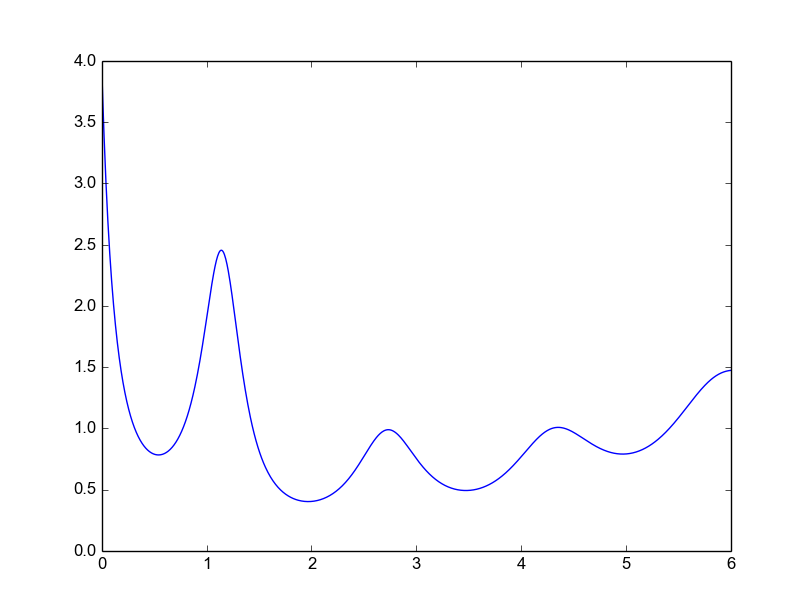
\includegraphics[width=\textwidth]{self_constructed_oned.png}
\end{minipage}
\end{frame}

%------------------------------------------------

\subsection{Results}

%------------------------------------------------
\begin{frame}
\frametitle{Results}
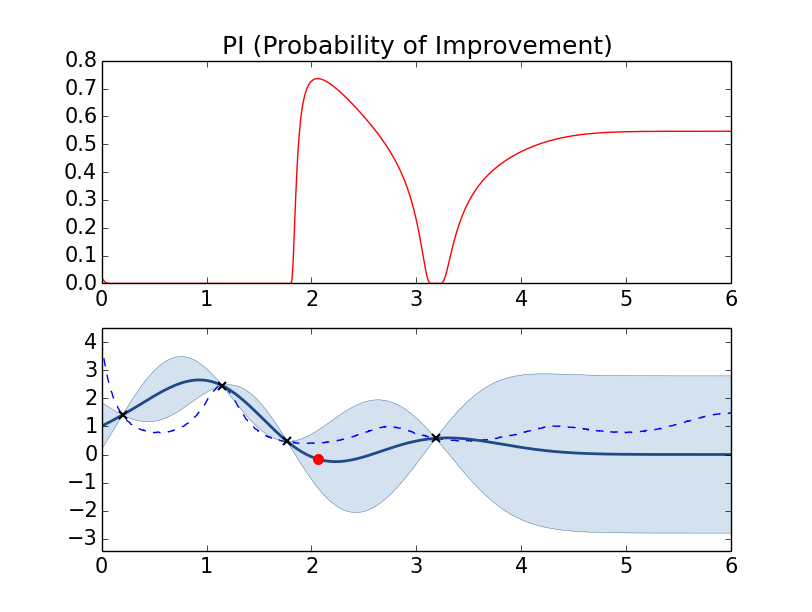
\includegraphics[width=\textwidth]{PI.png}
\end{frame}

%------------------------------------------------
\begin{frame}
\frametitle{Results}
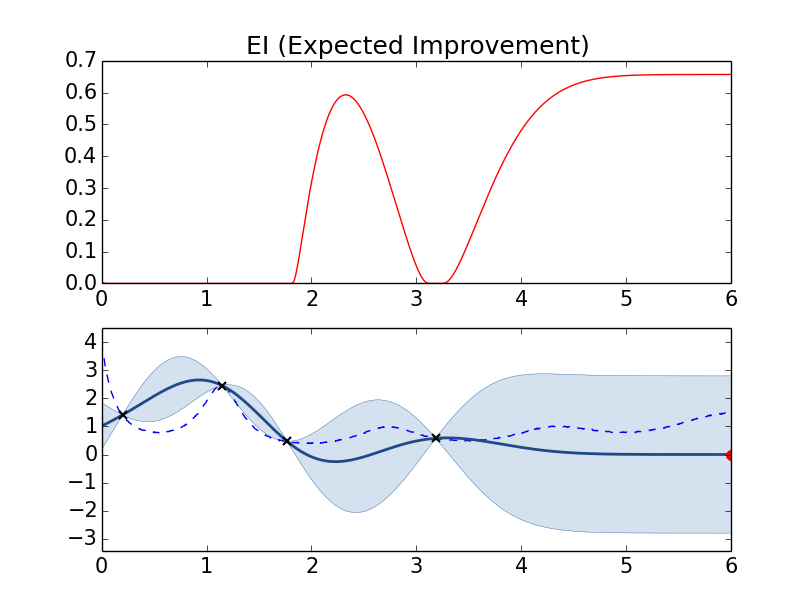
\includegraphics[width=\textwidth]{EI.png}
\end{frame}
%------------------------------------------------
\begin{frame}
\frametitle{Results}
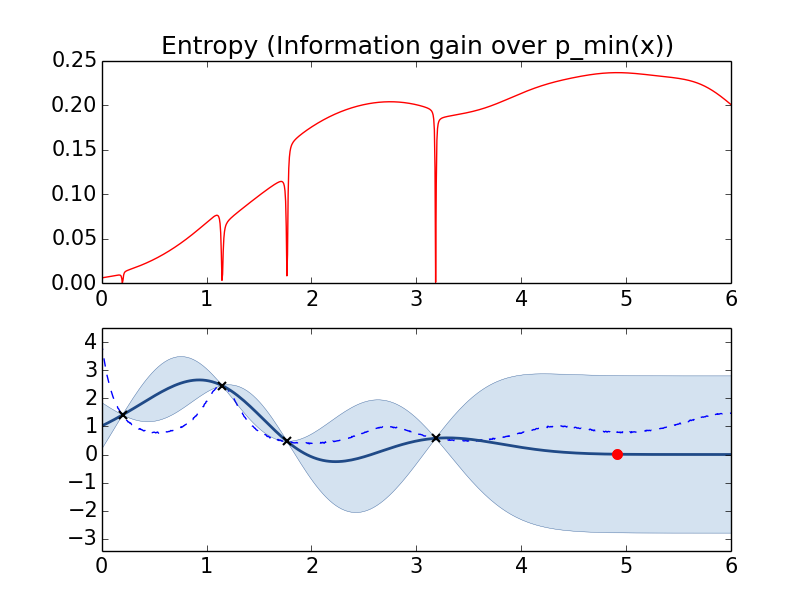
\includegraphics[width=\textwidth]{Entropy.png}
\end{frame}
%------------------------------------------------
\begin{frame}
\frametitle{Results}
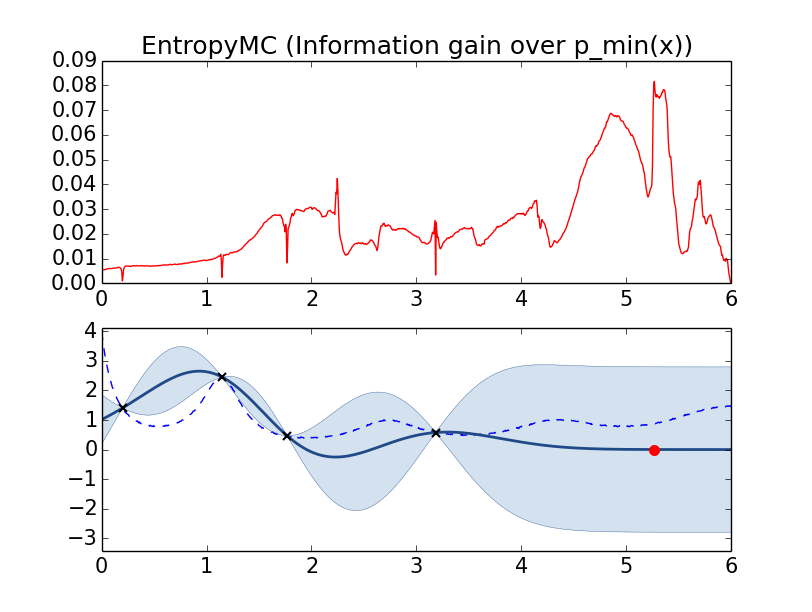
\includegraphics[width=\textwidth]{EntropyMC.png}
\end{frame}
%------------------------------------------------

\subsection{Test Functions}
\begin{frame}
\frametitle{Test functions}
\begin{minipage}{0.55\textwidth}
\begin{itemize}
\item Branin function as objective:
\begin{itemize}
\item dimensions: 2
\item global minima: 3
\item runs: 200
\end{itemize}
\item Acquisition functions:
\begin{itemize}
\item Expected Improvement
\item Probability of improvement
\item Upper confidence bound
\item Entropy (Expectation Propagation)
\item Entropy (Monte Carlo)
\end{itemize}
\end{itemize}
\end{minipage}%
\begin{minipage}{0.43\textwidth}
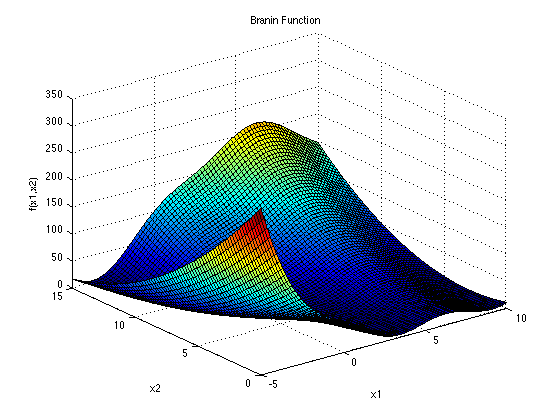
\includegraphics[width=\textwidth]{branin.png}
\end{minipage}
\end{frame}

\begin{frame}
\frametitle{Results}

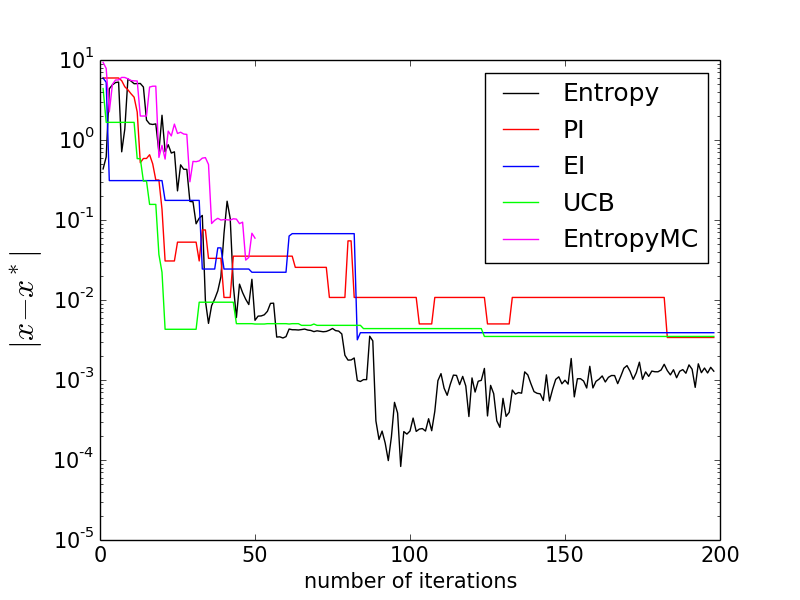
\includegraphics[width=\textwidth]{plot_branin2.png}

\end{frame}
%------------------------------------------------


%------------------------------------------------
\begin{frame}
\frametitle{Results}

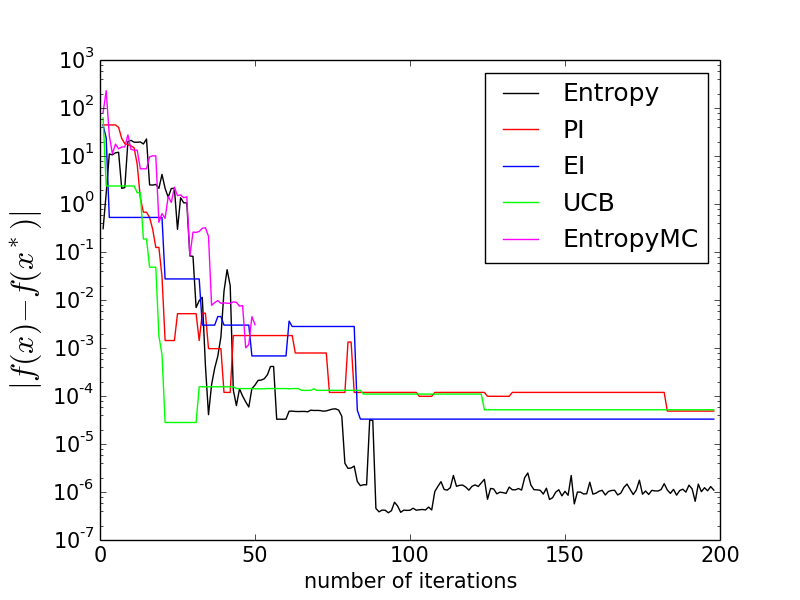
\includegraphics[width=\textwidth]{plot_branin1.png}

\end{frame}
%------------------------------------------------


\section{Conclusions}


%------------------------------------------------
\begin{frame}
\frametitle{Remarks}

\begin{itemize}[<+->]
	\item +
	\item -

\end{itemize}


\end{frame}


%------------------------------------------------
\begin{frame}
\frametitle{Future Directions}

\begin{itemize}
\item Support different kinds of parameters (conditional, categorial, continuous).
\item Can accept data set size as parameter.
\item Random Embeddings
\item Can change model if the current one performs poorly
\item Chooser: can access history, predictions can be forwarded
\end{itemize}

\end{frame}


%------------------------------------------------
%
%\begin{frame}
%\frametitle{References}
%\footnotesize{
%\begin{thebibliography}{99} % Beamer does not support BibTeX so references must be inserted manually as below
%%%%
%\bibitem[Hennig, 2011]{p1} Hennig, P.; Schuler, C. (2011)
%\newblock Entropy Search for Information-Efficient Global Optimization
%\newblock \emph{Proceedings of the Seventh Annual Symposium on Combinatorial
%Search (SoCS 20104)}.
%%%%%
%%\bibitem[birattari, 2010]{p1} Birattari, M. et al (2010)
%%\newblock F-race and iterated f-race: An overview.
%%\newblock \emph{Experimental Methods for the Analysis of Optimization 
%%Algorithms. Springer. 311-336}
%%%%%

%
%\end{thebibliography}
%}
%\end{frame}

%------------------------------------------------

%------------------------------------------------

%\begin{frame}
%\begin{center}
%\scalebox{10}{\textbf{?}}
%\end{center}
%\end{frame}

%------------------------------------------------



\begin{frame}
\Huge{\centerline{The End}}

\end{frame}

%----------------------------------------------------------------------------------------

			\end{document}
